\subsection{Multi-level Monte Carlo}

In this section, we will explain how to apply the Multi-level Monte Carlo method (MLMC) in this frame. Consider the approximation $U_k$ given by \eqref{probabilityODE} to the solution $u(t)$ of \eqref{ODE}. Given $\phi$ a function in $\mathcal C^\infty$, let us denote by $Z = \E(\phi(U_N)), Nh = T$ the expectation of the numerical solution at final time. If a standard Monte Carlo method over $M$ realizations of the numerical solution is applied, the only accessible quantity is
\begin{equation}\label{MonteCarlo}
	\hat Z = \frac{1}{M} \sum_{i = 1}^M \phi\left(U_N^{(i)}\right),
\end{equation}
where the index $i$ is referred to the $i$-th trajectory. Therefore, the quantity $\hat Z$ is an unbiased estimator of $Z$. Then, the Mean Square Error (MSE) of $\hat Z$ is given by
\begin{equation}\label{MSEMC}
\begin{aligned}
	\MSE(\hat Z) &= \E\left(\hat Z - \phi\left(u(T)\right)\right)^2 \\
	&= \Var\left(\hat Z\right) + \left(\E\left(\hat Z - \phi\left(u(T)\right)\right)\right)^2 \\
	&= \frac{C_1}{M} + C_2 h^{2\min\{2p, q\}},
\end{aligned}
\end{equation} 
where we have used Proposition \ref{thm:weakorder} with $C_1, C_2$ positive constants. If we introduce as a measure for the error 
\begin{equation}
	e = \sqrt{\MSE\left(\hat Z\right)},
\end{equation}
then in order to have $e = \OO(\epl)$, with $\epl$ fixed, one has to set
\begin{equation}
	h = \OO\left(\epl^{1 / \min\{2p, q\}} \right), \quad M = \OO(\epl^{-2}).
\end{equation}
If we measure the cost as the product between the number of timesteps and the number of trajectories, we find easily that in this case
\begin{equation}
	\mathrm{cost} = \OO\left(\epl^{-2 - 1/\min\{2p, q\}}\right).
\end{equation}
The idea of MLMC is introducing an \textit{hierarchical sampling}, introducing levels $l = 0, \ldots, L$, which have time step $h_l = T / N^l$ with $N_l = 2^l$. For each level, the number of trajectories is variable and is denoted by $M_l$. The estimator of $Z$ is then constructed as
\begin{equation}
	\bar Z = \sum_{l=0}^L \frac{1}{M_l} \sum_{i = 1}^{M_l}\left( \phi_l^{(i)} - \phi_{l-1}^{(i)} \right), \quad \phi_{l}^{(i)} = \phi \left(U_{N_l}^{(i)}\right).
\end{equation}
The values $\phi_l^{(i)}$ are constructed under two assumptions
\begin{enumerate}
	\item $\phi_l^{(i)}$ and $\phi_{l-1}^{(i)}$, with $\phi_{-1} \defeq 0$, are constructed using the same Brownian path,
	\item $\phi_l^{(i)}, \phi_{l-1}^{(i)}$ and $\phi_l^{(j)}, \phi_{l-1}^{(j)}$ are independent for $i \neq j$.
\end{enumerate}
The internal sum in $\bar Z$ is a telescopic sum, hence
\begin{equation}
	\E(\phi_L) = \E(\bar Z).
\end{equation}
Then we can compute the MSE of $\bar Z$ as
\begin{equation}
\begin{aligned}
	\MSE(\bar Z) &= \E\left(\bar Z - \phi\left(u(T)\right)\right)^2 \\
	&= \Var\left(\bar Z\right) + \left(\E\left(\bar Z - \phi\left(u(T)\right)\right)\right)^2 \\
	&= \Var\left(\bar Z\right) + \left(\E\left(\phi\left(U_{N_L}\right) - \phi\left(u(T)\right)\right)\right)^2 \\
	&= \Var\left(\bar Z\right) + \OO \left(h_L^{2\min\{2p, q\}}\right).
\end{aligned}
\end{equation}
The variance is then computable as
\begin{equation}
	\Var(\bar Z) = \sum_{l=0}^L \frac{1}{M_l^2} \sum_{i=1}^{M_l} \Var\left( \phi_l^{(i)} - \phi_{l-1}^{(i)} \right) = \sum_{l=0}^L \frac{V_l}{M_l}.
\end{equation}
Thanks to Proposition \ref{thm:strongConv} it is possible to estimate $V_l$.
\begin{lemma} If $\phi$ is Lipschitz continuous then 
\begin{equation}
	 V_l \leq C h_l^{2\min\{p, q\}},
\end{equation}
with $C > 0$ is a constant independent of $h_l$.
\end{lemma}
\begin{proof} Let us recall that for any random variable $Y_1, Y_2$, it is true that
\begin{equation}
	 \Var(Y_1 + Y_2) \leq 2 \left(\Var(Y_1) + \Var(Y_2)\right).
\end{equation}
Let us consider now the case $l = 0$. In this case
\begin{equation}
	V_0 = \phi_0 - \phi_{-1} = \OO(1),
\end{equation}
as $h_0 = T$. For $l \geq 1$, thanks to the property of the variance above 
\begin{equation}
\begin{aligned}
	\Var(\phi_l - \phi_{l-1}) &= \Var\left(\phi_l - \phi\left(u(T)\right) + \phi\left(u(T)\right) - \phi_{l-1}\right) \\
		&\leq 2\left(\Var\left(\phi_l - \phi\left(u(T)\right)\right) + \Var\left(\phi_{l-1} - \phi\left(u(T)\right)\right)\right)
\end{aligned}
\end{equation}
Then, considering singularly the two terms and denoting by $K$ the Lipschitz constant of $\phi$
\begin{equation}
\begin{aligned}
	\Var\left(\phi_l - \phi\left(u(T)\right)\right) &\leq \E \left(\phi_l - \phi\left(u(T)\right)\right)^2  = \E \left(\phi(U_{N_l}) - \phi\left(u(T)\right)\right)^2 \\
			&\leq K^2 \E \left(U_{N_l} - u(T)\right)^2  \\
			&\leq K^2 \E\left|U_{N_l} - u(T)\right|^2 \leq Ch_l^{2\min\{p, q\}},
\end{aligned}
\end{equation}
where the last bound is given by Proposition \ref{thm:strongConv}.
\end{proof}
\noindent Therefore, the MSE is given by
\begin{equation}
	\MSE(\bar Z) = C_1 h^{2\min\{2p, q\}}_L + C_2 \sum_{l=0}^L \frac{h_l^{2\min\{p, q\}}}{M_l}.
\end{equation}
We would like those two terms to balance, therefore we choose $M_l$ as
\begin{equation}
	M_l = \frac{h_l^{2\min\{p, q\}}L}{h_L^{2\min\{2p, q\}}},
\end{equation}
as in this way 
\begin{equation}
	\MSE(\bar Z) = C_1 h^{2\min\{2p, q\}}_L + C_2 \frac{L+1}{L} h_L^{2\min\{2p, q\}} = \OO\left(h^{2\min\{2p, q\}}_L\right).
\end{equation}
Hence, if we use as a measure of the error
\begin{equation}
	e = \sqrt{MSE\left(\bar Z \right)},
\end{equation}
and imposing $e = \OO(\epl)$ for a fixed $\epl$, we get for the finest time step
\begin{equation} \label{hLeps}
	h_L = \OO\left(\epl^{1/\min\{2p, q\}}\right).
\end{equation}
Let us compute the cost with this choice of the parameters. Defining the cost as the product of the number of time steps and the number of trajectories, we find
\begin{equation}
	\mathrm{cost} = \sum_{l=0}^L N_l M_l = \sum_{l=0}^L \frac{T}{h_l} \frac{h_l^{2\min\{p,q\}}L}{h_L^{2\min\{2p, q\}}}.
\end{equation}
For a matter of clarity in the computation, we consider three different cases. 

\subsubsection*{Case 1: $q \leq p$}
In this case, $\min\{p, q\} = q$ and $\min\{2p, q\} = q$. Therefore
\begin{equation}
\begin{aligned}
	\mathrm{cost} &=  \sum_{l=0}^L \frac{T}{h_l} \frac{h_l^{2q}L}{h_L^{2q}} = \frac{TL}{h_L} \sum_{l=0}^L \left(\frac{h_l}{h_L}\right)^{2q-1} \\
	&= \frac{TL}{h_L} \sum_{l=0}^L 2^{(L-l)(2q-1)} = \frac{TL}{h_L} 2^{L(2q-1)} \sum_{l=0}^L 2^{-l(2q-1)} \\
	&\leq L2^{2qL}\frac{1}{1 - 2^{1-2q}} \leq 2 L 2^{2qL} = \OO\left(L h_L^{-2q}\right),
\end{aligned}
\end{equation}
where we have assumed $q \geq 1$ so that the geometric series converges. Hence, in order to satisfy $e = \epl$ considering that $h_L = T / 2^L$ and \eqref{hLeps} we can impose
\begin{equation}\label{LCaseOne}
	L = \left|\log_2\epl^{1/q}\right|,
\end{equation} 
and therefore the cost can be expressed as 
\begin{equation}
	\mathrm{cost} = \OO\left(\left|\log_2 \epl^{1/q}\right| \epl^{-2}\right).
\end{equation}

\subsubsection*{Case 2: $q \geq 2p$}
In this case, $\min\{p, q\} = p$ and $\min\{2p, q\} = 2p$. Therefore
\begin{equation}
\begin{aligned}
\mathrm{cost} &=  \sum_{l=0}^L \frac{T}{h_l} \frac{h_l^{2p}L}{h_L^{4p}} = \frac{TL}{h_L^{2p+1}} \sum_{l=0}^L \left(\frac{h_l}{h_L}\right)^{2p-1} \\
&= \frac{TL}{h_L^{2p+1}} \sum_{l=0}^L 2^{(L-l)(2p-1)} = \frac{TL}{h_L^{2p+1}} 2^{L(2p-1)} \sum_{l=0}^L 2^{-l(2p-1)} \\
&\leq \frac{L2^{2pL}}{h_L^{2p}}\frac{1}{1 - 2^{1-2q}} = \OO\left(L h_L^{-4p}\right),
\end{aligned}
\end{equation}
Hence, in view of \eqref{hLeps} we impose as before 
\begin{equation}
	L = \left|\log_2 \epl^{1/2p}\right|,
\end{equation}
therefore the final expression of the cost is
\begin{equation}
	\mathrm{cost} = \OO\left(\left|\log_2 \epl^{1/2p}\right| \epl^{-2}\right).
\end{equation}

\subsubsection*{Case 3: $p < q \leq 2p$}
In this case, $\min\{p, q\} = p$ and $\min\{2p, q\} = q$. Therefore
\begin{equation}
\begin{aligned}
\mathrm{cost} &=  \sum_{l=0}^L \frac{T}{h_l} \frac{h_l^{2p}L}{h_L^{2q}} = \frac{TL}{h_L^{2q - 2p+1}} \sum_{l=0}^L \left(\frac{h_l}{h_L}\right)^{2p-1} \\
&= \frac{TL}{h_L^{2q-2p+1}} \sum_{l=0}^L 2^{(L-l)(2p-1)} = \frac{TL}{h_L^{2q-2p+1}} 2^{L(2p-1)} \sum_{l=0}^L 2^{-l(2p-1)} \\
&\leq \frac{L2^{2pL}}{h_L^{2q-2p}}\frac{1}{1 - 2^{1-2q}} = \OO\left(L h_L^{2p-2q-2p}\right) = \OO\left(L h_L^{-2q}\right).
\end{aligned}
\end{equation}
Hence the number of levels is given by
\begin{equation}
	L = \left|\log_2 \epl^{1/q} \right|,
\end{equation}
and the computational cost is given by
\begin{equation}
\mathrm{cost} = \OO\left(\left|\log_2 \epl^{1/q}\right| \epl^{-2}\right).
\end{equation}
Let us remark that in practice the method \eqref{probabilityODE} is tuned so that $p = q$, as in this case neither the strong or the weak order are spoiled by the noise added to the model. Therefore, the first of the three cases presented above is of the highest interest. The plot in Figure \ref{fig:MLMCtheory} shows that in this case MLMC is particularly favorable with respect to Monte Carlo when the integrator has an order $q$ which is small (e.g., $q = 1$).

%\begin{figure}
%	\centering
%	\resizebox{0.6\linewidth}{!}{% This file was created by matlab2tikz.
%
%The latest updates can be retrieved from
%  http://www.mathworks.com/matlabcentral/fileexchange/22022-matlab2tikz-matlab2tikz
%where you can also make suggestions and rate matlab2tikz.
%
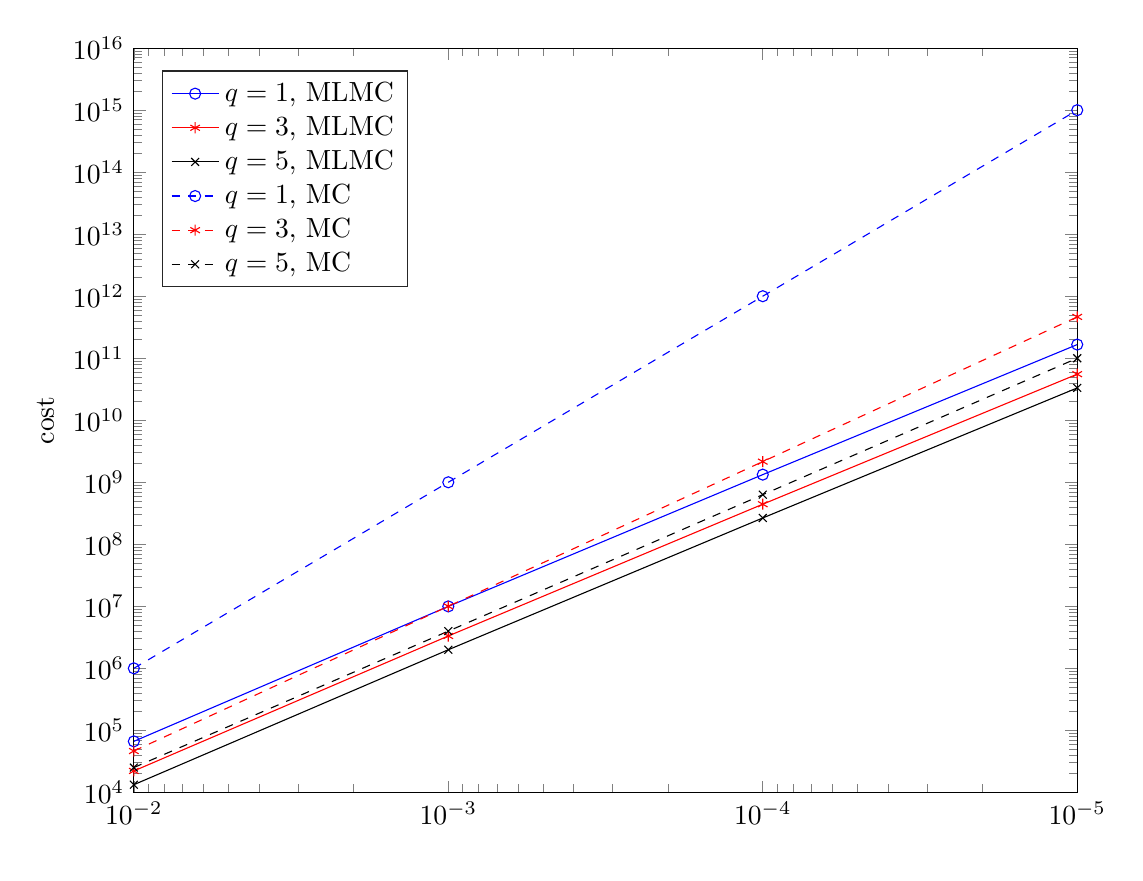
\begin{tikzpicture}

\begin{axis}[%
width=4.717in,
height=3.721in,
at={(0.791in,0.502in)},
scale only axis,
x dir=reverse,
xmode=log,
xmin=1e-05,
xmax=0.01,
xminorticks=true,
xlabel={$\epl$},
ymode=log,
ymin=10000,
ymax=1e+16,
yminorticks=true,
ylabel={cost},
axis background/.style={fill=white},
legend style={at={(0.03,0.97)},anchor=north west,legend cell align=left,align=left,draw=white!15!black}
]
\addplot [color=blue,solid,mark=o,mark options={solid}]
  table[row sep=crcr]{%
0.01	66438.5618977472\\
0.001	9965784.28466209\\
0.0001	1328771237.95494\\
1e-05	166096404744.368\\
};
\addlegendentry{$q = 1$, MLMC};

\addplot [color=red,solid,mark=asterisk,mark options={solid}]
  table[row sep=crcr]{%
0.01	22146.1872992491\\
0.001	3321928.09488736\\
0.0001	442923745.984982\\
1e-05	55365468248.1227\\
};
\addlegendentry{$q = 3$, MLMC};

\addplot [color=black,solid,mark=x,mark options={solid}]
  table[row sep=crcr]{%
0.01	13287.7123795495\\
0.001	1993156.85693242\\
0.0001	265754247.590989\\
1e-05	33219280948.8736\\
};
\addlegendentry{$q = 5$, MLMC};

\addplot [color=blue,dashed,mark=o,mark options={solid}]
  table[row sep=crcr]{%
0.01	1000000\\
0.001	1000000000\\
0.0001	1000000000000\\
1e-05	1e+15\\
};
\addlegendentry{$q = 1$, MC};

\addplot [color=red,dashed,mark=asterisk,mark options={solid}]
  table[row sep=crcr]{%
0.01	46415.8883361278\\
0.001	10000000\\
0.0001	2154434690.03189\\
1e-05	464158883361.279\\
};
\addlegendentry{$q = 3$, MC};

\addplot [color=black,dashed,mark=x,mark options={solid}]
  table[row sep=crcr]
%	\caption{Theoretical cost as a function of the desired accuracy and of the order $q$ of the numerical integrator if Monte Carlo or MLMC are applied.}
%	\label{fig:MLMCtheory}
%\end{figure}

%\subsubsection{Numerical example}
%We consider the Fitzhug-Nagumo problem \eqref{eq:FitzNag} and we aim to verify the cost of MLMC with respect to standard Monte Carlo for the estimation of the expectation of the solution at final time when applying the numerical method \eqref{probabilityODE}. We consider the case $q = p = 1$, using as a deterministic integrator the explicit Euler method. Hence, once a value of accuracy $\epl$ is requested, the number of stages $L$ as well as the time steps $h_l, l = 0, \ldots, L$, are imposed using \eqref{LCaseOne} and \eqref{hLeps}. In order to set up the standard Monte Carlo method, we consider the cost obtained in the MLMC simulation, denote by $\hat C$ and impose it to be equal for the standard Monte Carlo. In order to obtain a good balance between the error terms in \eqref{MSEMC} we impose
%\begin{equation}
%\begin{aligned}
%	\frac{T}{h} M &= \hat C, \\
%	M &= \ceil{h^{-2q}},
%\end{aligned}
%\end{equation}
%thus obtaining for the time step
%\begin{equation}
%	h = \left(\frac{T}{\hat C}\right)^{1 / (2q + 1)}.
%\end{equation}
%In this way, the computational cost for MLMC and standard Monte Carlo are imposed to be artificially equal and the two methods can be compared for their weak error with respect to an accurate solution. We impose for MLMC four values of accuracy $\epl = 0.1, 0.01, 0.001, 0.0001$, and apply the aforementioned technique to compare MLMC and Monte Carlo. Results (Figure \ref{fig:MLMCpractice}) show that imposing $L$ and $h_l, l = 0, \ldots, L$ as above the obtained accuracy in the same order of magnitude as $\epl$. Furthermore, the obtained accuracy is smaller for MLMC than MC if the cost 
%
%\begin{figure}
%	\centering
%	\resizebox{0.6\linewidth}{!}{% This file was created by matlab2tikz.
%
%The latest updates can be retrieved from
%  http://www.mathworks.com/matlabcentral/fileexchange/22022-matlab2tikz-matlab2tikz
%where you can also make suggestions and rate matlab2tikz.
%
\definecolor{mycolor1}{rgb}{0.00000,0.44700,0.74100}%
%
\begin{tikzpicture}

\begin{axis}[%
width=4.717in,
height=3.721in,
at={(0.791in,0.502in)},
scale only axis,
xmode=log,
xmin=100,
xmax=10000000000,
xminorticks=true,
xlabel={Cost},
ymode=log,
ymin=0.0001,
ymax=1,
yminorticks=true,
ylabel={Accuracy},
axis background/.style={fill=white},
legend style={legend cell align=left,align=left,draw=white!15!black}
]
\addplot [color=mycolor1,solid,mark=o,mark options={solid}]
  table[row sep=crcr]{%
480	0.25110925\\
56896	0.0261217025\\
5237760	0.002328838\\
1878933504	0.000163954625\\
};
\addlegendentry{MLMC};

\addplot [color=red,solid,mark=o,mark options={solid}]
  table[row sep=crcr]
%	\caption{Accuracy of MLMC and standard Monte Carlo for the FitzHug-Nagumo problem with fixed cost.}
%	\label{fig:MLMCpractice}
%\end{figure}